\section{Step 5: install the 3D-printed holders}\label{sec:walk-printed}
These holders are ours (not Stanford's): they put the amplifier and both supplies on the tower profile
instead of on the floor or on tape. If you build a tower from scratch, you can mount them before the
cabling. Files: \file{hardware/enclosures/out/}; overview with pictures and mounting steps:
\file{hardware/enclosures/out/fit_check.pdf} and \file{parts-overview.pdf}.

\subsection{Print}
\begin{enumerate}
\item PETG or ASA, no supports, brim recommended; the two holders stand on their end.
\item Print \file{fit_check.stl} first: one test plate and one of each holder on one bed (157$\times$51\,mm).
\item Push the test plate into a profile slot. It should slide in without play. If it is too tight or loose,
print \file{test_fit.stl} (clearance 0.1 / 0.2 / 0.3\,mm per side, marked with 1 / 2 / 3 notches), set
\cmd{KEY\_CLEAR} in \file{tower.py} to the best one and run \cmd{python make\_stl.py} again.
\item Print one set per tower: \file{iaa100_din_mount.stl}, \file{rs15_plate.stl},
\file{rsp2000_brackets.stl} (bracket A and B). The 48\,V supply weighs 1.95\,kg and gets warm: its brackets in
ASA, or PETG with at least 40\,\% infill.
\end{enumerate}

\subsection{Install}
\begin{table}[H]\centering\small
\begin{tabularx}{\linewidth}{lXl}
\toprule
Holder & Device & Screws \\
\midrule
DIN-rail mount & Futek IAA100 clips onto the printed 35\,mm rail & M6 into the profile \\
RS-15 plate & Mean Well RS-15-24, 2$\times$ M3$\times$6 from the back & M6 into the profile \\
RSP-2000 brackets & one at each end of the RSP-2000-48: A with 2$\times$ M4$\times$12, B with 1$\times$ M4$\times$12; 10\,mm air gap behind the supply & M6 into the profile \\
\bottomrule
\end{tabularx}
\end{table}
\begin{enumerate}
\item Supplies \textbf{unplugged}. Fit the device to its holder first, then the holder to the profile.
\item Profile screws: M6 ISO~7380 button heads in slot-10 T-nuts, at least about 5\,mm of thread in the
T-nut (probably M6$\times$16; confirm on the test print).
\item The 48\,V supply: two people, fan ends free.
\item Remove the old tape.
\end{enumerate}
\textbf{Check:} push each device by hand: nothing moves; the supply's fans are not blocked.

\begin{figure}[H]\centering
\begin{minipage}{0.32\linewidth}\centering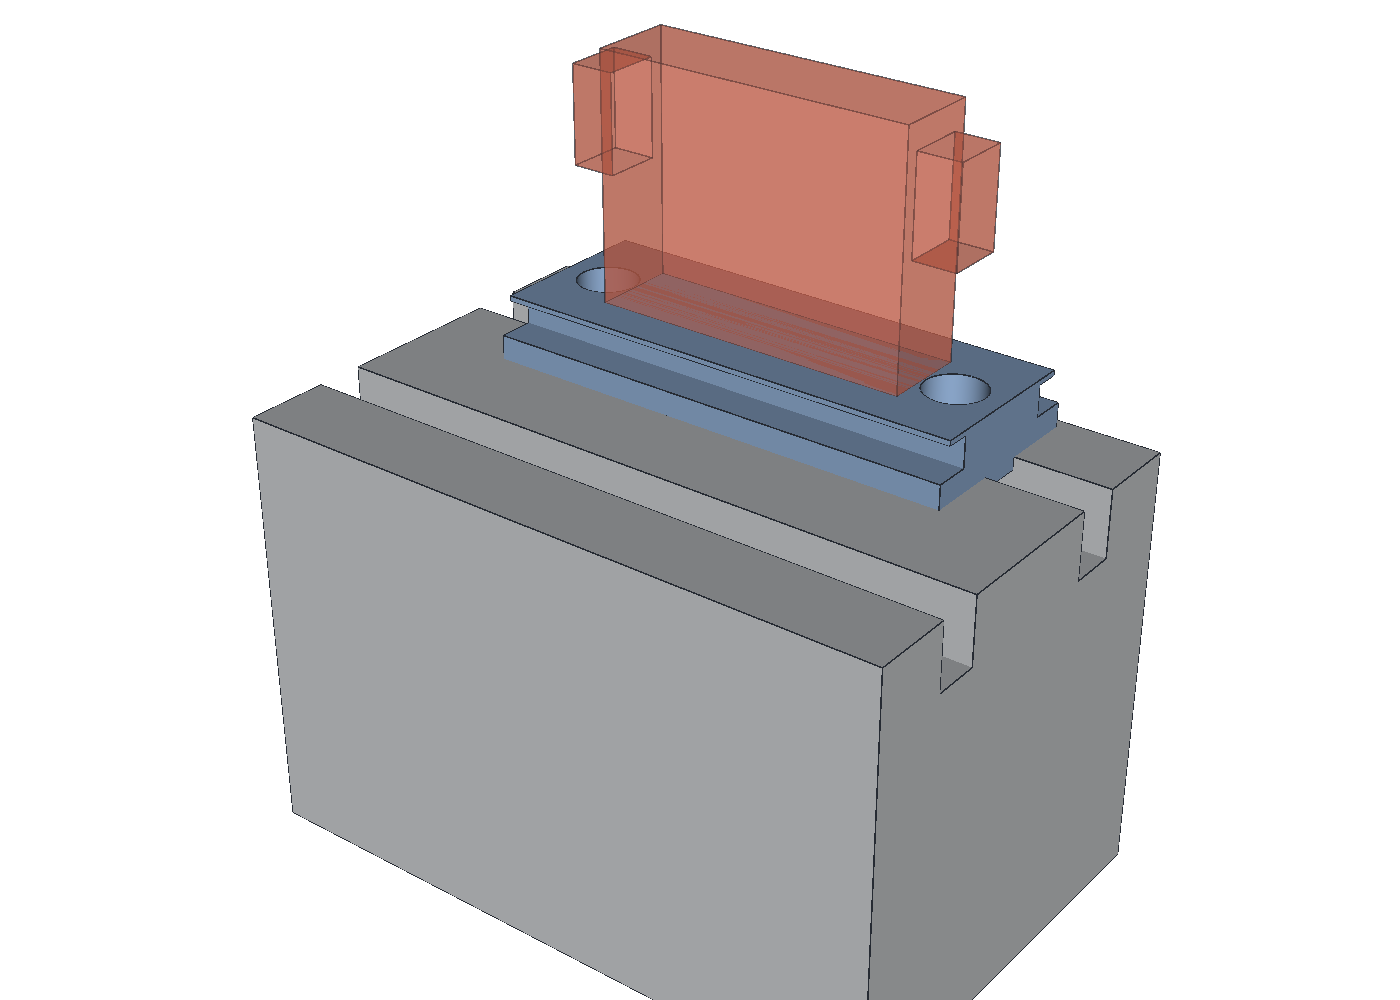
\includegraphics[width=\linewidth]{figures/render-iaa100.png}\\\scriptsize IAA100 on its DIN rail\end{minipage}\hfill
\begin{minipage}{0.32\linewidth}\centering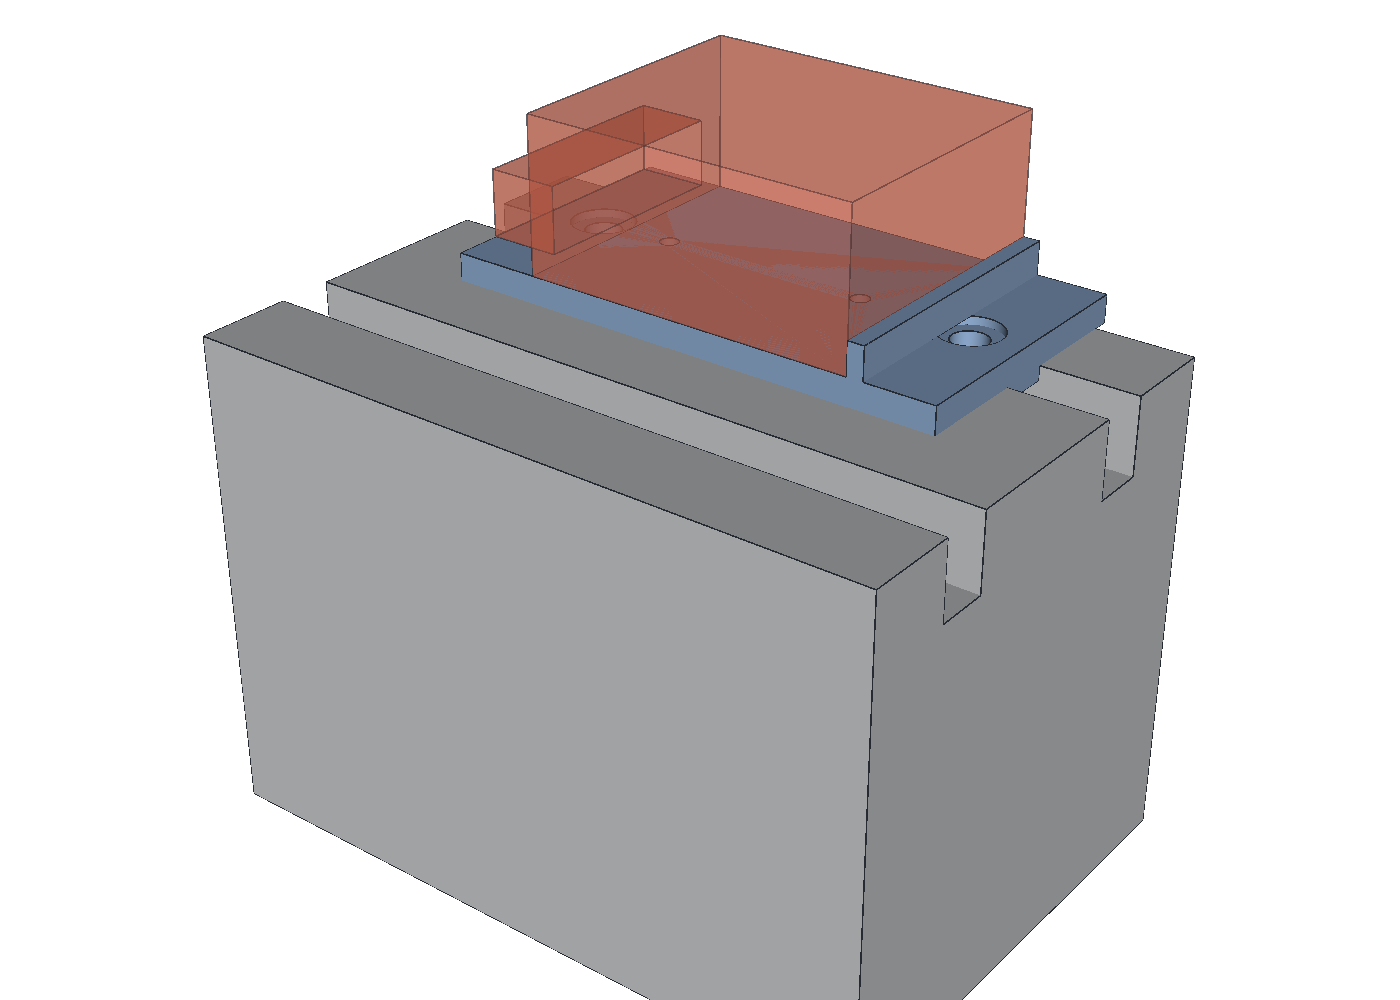
\includegraphics[width=\linewidth]{figures/render-rs15.png}\\\scriptsize RS-15-24 on its plate\end{minipage}\hfill
\begin{minipage}{0.32\linewidth}\centering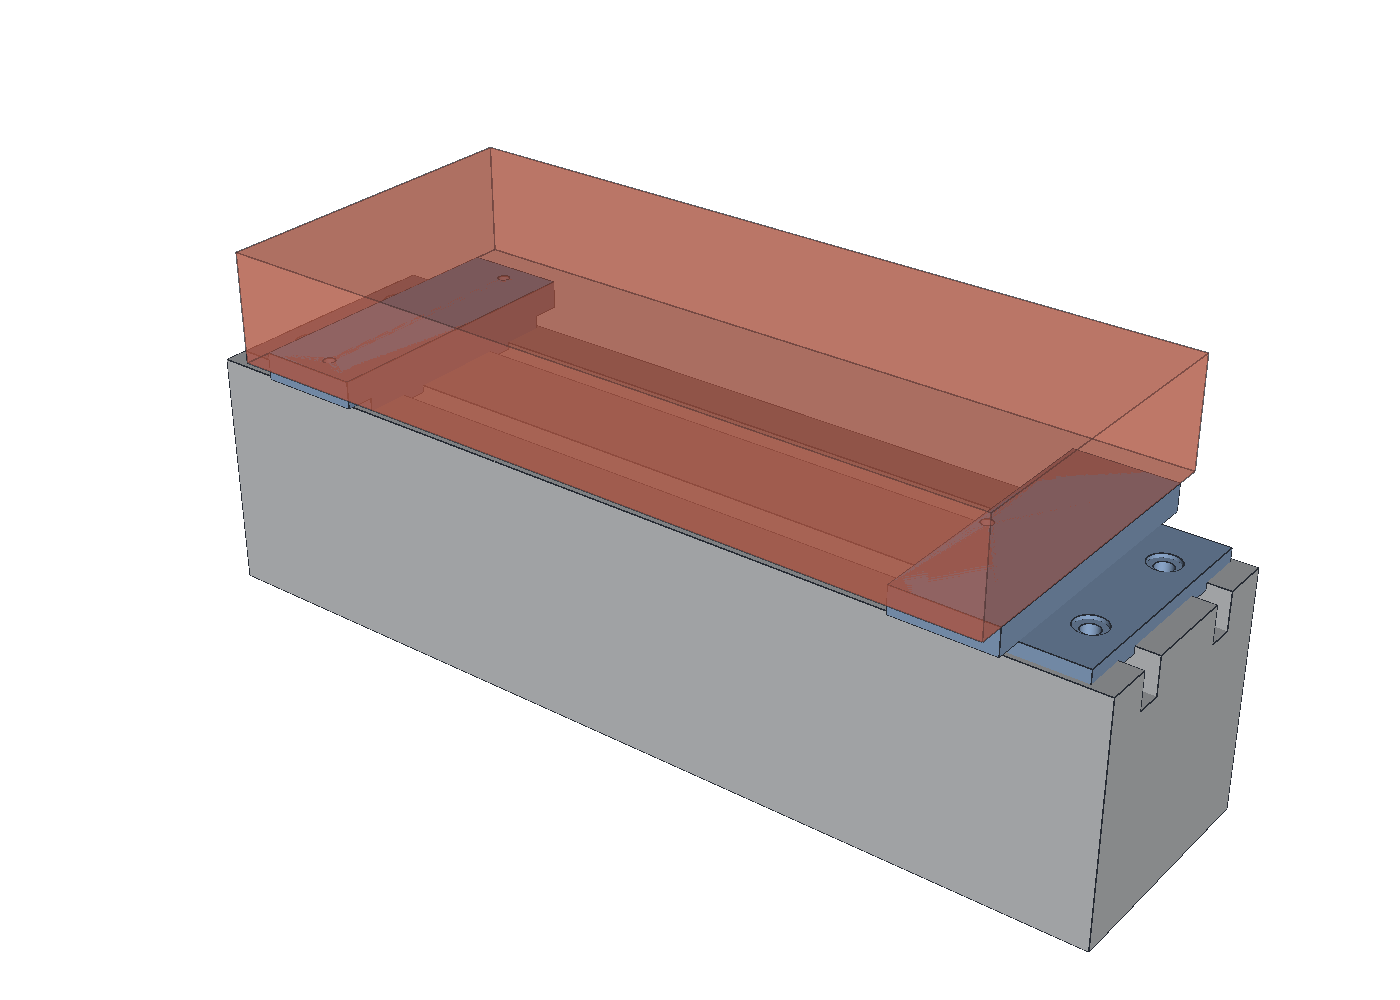
\includegraphics[width=\linewidth]{figures/render-rsp2000.png}\\\scriptsize RSP-2000 in its brackets\end{minipage}
\end{figure}
